% !TEX root = ../intro-stellar-physics.tex

\nocite{Mihalas1978Stellar-Atmosph,LeBlanc2010An-Introduction,Carroll2006An-Introduction}

To recap, we have established a description for the basic features of self-gravitating fluid:
\begin{enumerate}

\item For a set mass and radius, hydrostatic equilibrium (balance of pressure and gravity) is established on the time needed for a sound wave to cross the star. Once this equilibrium is established, the central pressure, density, and temperature are established.

\item The gradient in temperature from center to surface drives a luminosity, which is controlled by the opacity of material in the stellar interior.

\item The ambient pressure and temperature near the stellar photosphere (where $\tau \sim 1$) are set by the surface gravity and opacity.

\end{enumerate}

What we haven't---yet---established is how the luminosity is generated: if nuclear reaction are not operating, then the star must contract (on a Kelvin-Helmholtz timescale) until the central temperature is sufficiently hot for reactions to generate the required luminosity.
Before discussing this, however, we shall explore how the emergent spectra of stars serve as diagnostic indicators of ambient conditions in the stellar photosphere. 

\section{Overview}

If light from the Sun is passed through a grating (a piece of glass with finely etched lines), the light is dispersed in wavelength and creates a spectrum, such as the highly detailed one show in Fig.~\ref{f.solar-spectrum}. 
\begin{marginfigure}
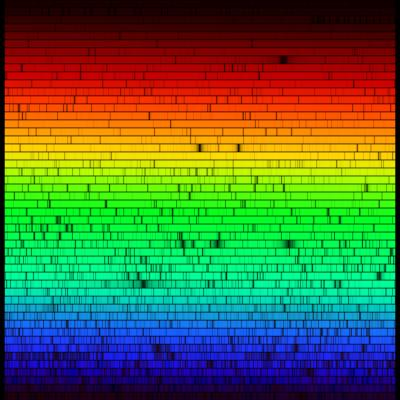
\includegraphics[width=\linewidth]{sunsqa}
\caption{\label{f.solar-spectrum} Visible spectrum of the Sun. Wavelength increases along a row from left to right, and by rows from bottom to top. \emph{Credit:
N.A.Sharp, NOAO/NSO/Kitt Peak FTS/AURA/NSF. Image copyright }}
\end{marginfigure}
Superposed on the slow variation from red to violet are dark \newterm{absorption lines}. These are caused by absorption of photons at specific frequencies by ions, atoms, and molecules in the solar atmosphere.

Beginning in the late 1800's, astronomers began classifying stars by the observed absorption lines in the spectra. At this time, Edward Pickering and Williamina Fleming of the Harvard College Observatory began amassing a vast catalog of stellar spectra. They classified these spectra according to the strength of observed hydrogen Balmer lines (the first four are H$\alpha$: \val{657}{\nano\meter}; H$\beta$: \val{486}{\nano\meter}; H$\gamma$: \val{434}{\nano\meter}; H$\delta$: \val{410}{\nano\meter}). Stars, such as Vega, with the strongest Balmer lines were classified as type ``A'', those with the next strongest were type ``B'', and so forth. In Annie Jump Cannon, who had joined the group in 1896 and would later succeed Fleming as curator of astronomical photography at the observatory, simplified and reorganized the scheme, and added decimal subdivisions ($0\ldots9$) for each type\sidenote{For example, the Sun's type is G2}. When stellar color is taken into account, the ordering of stars, from blue to red, is ``OBAFGKM''. In the 1990's the ``L'' and ``T'' classes were added\cite{Kirkpatrick1999Dwarfs-Cooler-t} for cool stars and brown dwarfs (stellar-like objects that do not reach central temperature sufficient for fusion of hydrogen into helium).

Hertzsprung and Russell independently noticed that most stars tended to lie along a band, termed the \newterm{main sequence} in a plot of absolute magnitude (or luminosity) against stellar type (now known as a \newterm{Hertzsprung-Russell diagram}). Figure~\ref{f.HR} shows some standard main-sequence stars, along with their stellar type and approximate color.
\begin{marginfigure}
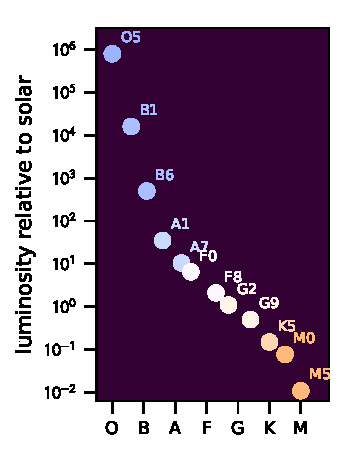
\includegraphics[width=\linewidth]{HR}
\caption{\label{f.HR} Hertzsprung-Russell diagram showing standard main-sequence stars. Colors are approximate translations of the spectra.}
\end{marginfigure}

In an influential PhD thesis, Cecilia Payne-Gaposhkin\cite{Payne1925Stellar-Atmosph} applied the Boltzmann and Saha equations to show that different stellar spectra were consistent with changes in temperature, rather than composition, of the stellar photosphere. The sequence of stellar types is therefore a temperature sequence, with ``O'' stars being the hottest. 

\section{The hydrogen atom}

To understand why the Balmer lines are strongest in a certain range of temperatures, we first need to review the workings of a hydrogen atom.

The electrons bound to an atom or molecule can only occupy states having a discrete set of energies. For example, the electron in a hydrogen atom only has energies
\begin{equation}\label{e.H-levels}
        E_{n} = -\val{13.6}{\eV}\times \frac{1}{n^{2}},
\end{equation}
where $n > 0$ is an integer known as the principal quantum number.  These energies are negative, relative to a free electron.  For example, the ground state ($n=1$) has energy $\ERy = -\val{13.6}{\eV}$, meaning that it takes \val{13.6}{\eV} to remove an electron in its ground state from the atom.

Because the electrons in an atom can only have certain energies, the atom can only absorb or emit light at specific wavelengths, such that the energy of the photon matches the difference in energy between two levels. For example, a hydrogen atom in its ground state can absorb a photon of energy
\[
        E_{1\to2} = -\ERy \left(\frac{1}{2^{2}} - \frac{1}{1^{2}}\right)
                 = \val{10.2}{\eV}
\]
corresponding to the energy required to move the electron from $n=1$ to $n=2$. The wavelengths that can be absorbed by a hydrogen atom at rest can be found by substituting $E = hc/\lambda$ into equation~(\ref{e.H-levels}):
\begin{equation}
        \lambda_{m\to n} = \lambda_{0}\left(\frac{1}{n^{2}}-\frac{1}{m^{2}}\right)^{-1},
\end{equation}
where $\lambda_{0} = \val{91.2}{\nano\meter}$ and $n > m$.
The transitions to the lowest levels are named after their discoverers: Lyman for $m\to1$, Balmer for $m\to2$, Paschen for $m\to3$. A greek letter is used to denote the higher state: for example Lyman $\alpha$ (abbr.\ Ly$\alpha$) means $2\to1$, with $\lambda_{\mathrm{Ly}\alpha} = \val{121.6}{\nano\meter}$.  The first line transition in the Balmer series is $3\to2$, and is designated H$\alpha$: $\lambda_{\mathrm{H}\alpha} = \val{656.3}{\nano\meter}$. The first 20 lines for the Lyman ($m\to1$), Balmer ($m\to2$), and Paschen ($m\to3$) are shown in Fig.~\ref{f.H-spectrum}; note the $4\to3$ transition is outside the plot range. The Balmer lines lie in the visible range. Note that $\lambda_{m\to n} < \lambda_{0}$; photons with wavelengths $\lambda < \val{91.2}{\nano\meter}$ have sufficient energy to knock the electron out of the atom, thereby producing a hydrogen ion and a free electron.

\begin{marginfigure}[-8\baselineskip]
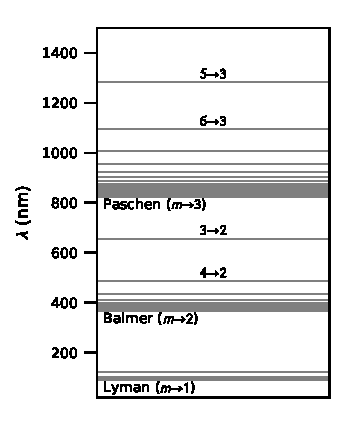
\includegraphics[width=\linewidth]{H-spectrum}
\caption{Spectral lines of neutral hydrogen. 
\label{f.H-spectrum}}
\end{marginfigure}

\section{The Boltzmann Equation}
\label{s.boltzmann-eqn}

In order to produce a Balmer absorption line, we must have some hydrogen atoms in the photosphere with electrons in the energy level $n=2$. The more atoms with $n=2$, the more absorption and the stronger the line. To find the number of atoms with energy level $n=2$, we make use of a fundamental result, due to Boltzmann, from statistical (thermal) physics; namely, that if our sample of atoms is in thermal equilibrium, then the ratio of the number of atoms with energy $E_{i}$ to the number of atoms with energy $E_{j}$ is
\begin{equation}\label{e.boltzmann}
\frac{N_{i}}{N_{j}} = \frac{g_{i}}{g_{j}} 
\exp\left(-\frac{E_{i}-E_{j}}{\kB T}\right).
\end{equation}
Here the number $g_{n}$ gives the number\sidenote{$g_{n}$ is known as the \emph{degeneracy} of a given level $n$} of quantum mechanical states having energy $E_{n} = -\ERy/n^{2}$. For an energy level $n$, there are $n^{2}$ possible states, each having a different angular momentum. For each of these $n^{2}$ states, both the electron and proton may each have 2 possible spins. The total number of states for energy $E_{n}$ is therefore $g_{n} = 2\times2\times n^{2}$.

Suppose we wish to know the fraction of atoms in a given state $i$: that is, we want to know
\[	x_{i} = \frac{N_{i}}{N_{1}+N_{2}+\ldots+N_{i}+\ldots} ? \]
Using equation~(\ref{e.boltzmann}), we can express $x_{i}$ as 
\begin{eqnarray}
  x_{i} &=& \frac{g_{i}e^{-E_{i}/\kB T}}{g_{1}e^{-E_{1}/\kB T}+g_{2}e^{-E_{2}/\kB T}+\ldots+g_{i}e^{-E_{i}/\kB T}+\ldots} \nonumber\\
        &\equiv& \frac{g_{i}e^{-E_{i}/\kB T}}{\pfcn}.
\end{eqnarray}
The quantity 
\begin{equation}\label{e.partition-function}
	\pfcn = \sum_{n} g_{n}\exp\left(-\frac{E_{n}}{\kB T}\right)
\end{equation}
is called the \emph{partition function}: loosely speaking, it indicates the number of ways the sample of atoms can be partitioned among the different energy levels.

\begin{exercisebox}[Partition function for neutral hydrogen]
Assuming that the first term $g_{1}e^{-E_{1}/\kB T}$ dominates the sum in the partition function (see Box~\ref{sb.partition-function}), plot the fraction of neutral hydrogen in its $n=2$ state as a function of temperature, for $\val{5\,000}{\K} < T < \val{20\,000}{\K}$.
\end{exercisebox}

\begin{sidebar}[The partition function for neutral hydrogen]
\label{sb.partition-function}
The partition function for neutral hydrogen, eq.~(\ref{e.partition-function}), has some interesting features. Substituting $g_{n}=4n^{2}$ and $E_{n} = -\ERy/n^{2}$ and factoring out common terms gives,
\[	\pfcn = 4e^{\beta\ERy}\sum_{n} n^{2} e^{-\beta\ERy(1-1/n^{2})}. \]
Here we have used the shorthand $\beta = (\kB T)^{-1}$. Written in this fashion, it is clear that for $n\gg 1$, the sum diverges, since the individual terms go as $n^{2}e^{-\beta\ERy}$ as $n\to\infty$. In practice, this isn't a problem, as there is an upper limit on $n$ set by ambient conditions. For example, the mean distance of the electron from the nucleus is $\approx \abohr n^{2}$, where $\abohr = \val{\sci{5.29}{-11}}{\cm}$ is the Bohr radius. As a result, each atom takes up a volume $\approx \abohr^{3}n^{6}$; if we want the atoms to not overlap, then the volume per atom, $V/N = 1/xi$, must be larger than this by some factor. Suppose we set that the volume of an atom must be less than half of that available in our gas; then
\[
\xi = \frac{N}{V} < \frac{N}{N\cdot 2\abohr^{3}n^{6}}.
\]
Thus the maximum level is $n < (2\abohr^{3}\xi)^{-1/6}$. For a typical A-star photospheric density $\xi\sim \val{10^{15}}{\cm^{-3}}$, the density cutoff is $n \lesssim 35$. In practice the cutoff will be even lower.

The precise maximum value of $n$ is not that important for most applications. The reason is that the in the partition function increase only slowly. For example, at $T=\val{10^{4}}{\K}$, the terms and cumulative sum in the partition function are as follows.
\begin{center}
\begin{tabular}{rrr}
$n$ & $n^{2} e^{\beta\ERy(1-1/n^{2})}$ & $4\sum_{i=1}^{n} i^{2}e^{-\beta\ERy(1-1/i^{2})}$ \\
\hline
   1 & 1.00e+00 &  4.0000 \\
   2 & 2.88e-05 &  4.0001 \\
   3 & 7.23e-06 &  4.0001 \\
  \multicolumn{3}{c}{\vdots} \\
  26 & 9.62e-05 &  4.0038 \\
  \multicolumn{3}{c}{\vdots} \\
  52 & 3.78e-04 &  4.0274 \\
  \multicolumn{3}{c}{\vdots} \\
 268 & 9.99e-03 &  7.5901 \\
\end{tabular}
\end{center}
As we can see from the cumulative sum (rightmost column), the partition function is insensitive to the precise value of the cutoff; indeed, it is reasonably accurate to just use the first term, $Q\approx 4e^{\beta\ERy}$. 
\end{sidebar}

\section{Ionization: The Saha equation}
\label{s.saha-eqn}

As the temperature in the gas rises, there are more photons with sufficient energy to eject electrons from an atom. In addition, collisions between atoms also become sufficiently energetic to ionize the atom. In astronomical nomenclature, the ionization state is denoted by a small Roman numeral: \ion{Fe}{i} denotes neutral iron, \ion{Fe}{ii} denotes singly-ionized iron (charge $+1$), \ion{Fe}{iii} denotes doubly-ionized iron (charge $+2$), and so on. In thermal equilibrium, the rate at which atoms are ionized must equal the rate at which ions and electrons recombine: for example, in a gas consisting of hydrogen atoms, hydrogen ions (i.e., protons), and electrons the reaction
\[
	\ion{H}{ii} + e \longleftrightarrow \ion{H}{i}
\]
is in equilibrium. We'd like to extend equation~(\ref{e.boltzmann}) to find the ratio of two ionization states $N_{i+1}/N_{i}$. Although deriving this equation, termed the \newterm{Saha equation}\sidenote{Derived by Meghnad Saha in 1920}, is beyond the scope of the course, what we shall do is take the equation apart and try to understand how it works.  The Saha equation for the ratio of two ionization states $N(i+1)$ and $N(i)$ is
\begin{equation}\label{e.saha}
\frac{N_{i+1}}{N_{i}} 
= {\color{red}\left[\frac{2}{n_{e}}
\left(\frac{2\pi m_{e}\kB T}{h^{2}}\right)^{3/2}\right]}
{\color{blue}\frac{\pfcn_{i+1}}{\pfcn_{i}}}.
\end{equation}
In this equation, $n_{e}$ denotes the electron density---the number of free electrons per unit volume---and $m_{e}$ is the electron mass. The terms $\pfcn_{i+1}$ and $\pfcn_{i}$ are the partition functions for the two states, \emph{both measured with the same zero-point for energy}.

Let's start with the term $\color{blue} Q_{i+1}/Q_{i}$. If both partition functions are dominated by the ground state term\sidenote{see Box~\ref{sb.partition-function}} then
\begin{eqnarray*}
	\frac{Q_{i+1}}{Q_{i}} &=& \frac{g_{i+1,1}}{g_{i,1}} e^{-\beta (E_{i+1,1}-E_{i,1})}\\
	&=& \frac{g_{i+1,1}}{g_{i,1}} e^{-\beta\,E_{\mathrm{ion}}}
\end{eqnarray*}
Here $E_{\mathrm{ion}} = E_{i+1,1} - E_{i,1}$ is the energy needed to remove an electron from an ion in state $i$. Thus $Q_{i+1}/Q_{i}$ resembles equation~(\ref{e.boltzmann}).

The term in $\color{red}\left[\cdot\right]$ in eq.~(\ref{e.saha}) arises because we also need to allow for the number of possible electron states. When the atom is ionized, each electron quickly acquires an average kinetic energy $(3/2)\kB T$. There are many different states with this energy: the electron can be in different locations and moving in different directions.  You might think that there would be an infinitude of possible electron states.  Quantum mechanics, however, sets limitations on this number.

First, we have the Pauli exclusion principle: no two electrons can be in the same location with the same momentum and same spin. What do we mean by same location and momentum?  Recall the Heisenberg uncertainty principle: the electrons $x$-position and $x$-momentum are spread about a range of values $\Delta x$ and $\Delta p_{x}$, and these uncertainties are related via
\[ \Delta x\,\Delta p_{x} \gtrsim h. \]
Thus, if we imagine dividing our volume into little boxes of volume
\[ 
 \Delta V = \Delta x\,\Delta y\,\Delta z \approx \frac{h^{3}}{\Delta p_{x}\,\Delta p_{y}\,\Delta p_{z}},
\]
each box can hold two electrons.\sidenote{Because electrons have spin 1/2, we can put two electrons into the same position and momentum state if their spins are oppositely directed.} Suppose we have a volume $V$; how many boxes are there?  The number of available boxes is
\[
	\frac{V}{\Delta V} \approx \frac{V\;\Delta p_{x}\,\Delta p_{y}\,\Delta p_{z}}{h^{3}}.
\]
To estimate the size of $\Delta p_{x}\,\Delta p_{y}\,\Delta p_{z}$, let's estimate $\Delta p_{x}\sim p_{x}$; further, if everthing is isotropic then $p_{x}\approx p_{y}\approx p_{z}$ on average, so $\Delta p_{x}\,\Delta p_{y}\,\Delta p_{z} \sim p_{x}^{3}$.  Now the kinetic energy of the electron is $p^{2}/2m_{e}$, and $p^{2} = p_{x}^{2} + p_{y}^{2} + p_{z}^{2} \approx 3 p_{x}^{2}$. Hence the kinetic energy is $(3/2)p_{x}^{2}/m_{e}$; in thermal equilibrium, however, the kinetic energy has an average value of $(3/2)\kB T$.  The value of $p_{x}^{2}$ is therefore
\[
	p_{x}^{2} \approx m_{e}\kB T,
\]
and the number of boxes is
\[
	\frac{V}{\Delta V} \sim V\frac{p_{x}^{3}}{h^{3}} \sim V\frac{\left(m_{e}\kB T\right)^{3/2}}{h^{3}}.
\]
If our volume $V$ contains $N_{e}$ electrons, then the number of boxes---which is the number of states---per electron is
\[
	\frac{2V}{N_{e}\Delta V} \sim \frac{2V}{N_{e}}\frac{\left(m_{e}\kB T\right)^{3/2}}{h^{3}}.
\]
The factor of 2 appears because each box can hold 2 electrons.  Recognizing that $N_{e}/V = n_{e}$, we see that this number of states per free electrons corresponds to the factor in $\color{red}\left[\;\right]$ in equation~(\ref{e.saha}). When the numerical calculation is done correctly, the additional factor of $2\pi$ arises.

The number of states per free electron plays an important role in setting the temperature at which a species ionizes. You might expect, since a term $e^{-E_{\mathrm{ion}}/\kB T}$ appears in the ratio $N_{i+1}/N_{i}$, that a species would ionize at a temperature $E_{\mathrm{ion}}/\kB$. In fact the ionization temperature is much lower. To see how this works, define
\[
	\zeta = \ln\left[\frac{1}{n_{e}}\left(\frac{2\pi m_{e}\kB T}{h^{2}}\right)^{3/2}\right].
\]
We can then write eq.~(\ref{e.saha})---with the approximation that the partition functions are dominated by the ground state---as
\[
	\frac{N_{i+1}}{N_{i}} = \frac{2g_{i+1,1}}{g_{i,1}}\exp\left(\zeta - \beta E_{\mathrm{ion}}\right).
\]
Now the factor $g_{i+1,1}/g_{i,1}$ is of order unity. Hence, when the gas ionizes and $N_{i+1,1}\approx N_{i,1}$, we must have that $\zeta\approx \beta E_{\mathrm{ion}}$; put differently, the ionization temperature will not be $E_{\mathrm{ion}}/\kB$ but rather $E_{\mathrm{ion}}/\kB\zeta$. Under conditions in the photosphere of an A star ($T \approx \val{10^{4}}{\K}$, $n\sim \val{10^{15}}{\cm^{-3}}$), $\zeta \approx 15$.


\section{Classifying stars by spectra}

The Balmer lines, which correspond to transitions $2\to3$, $2\to 4$, \ldots, are most prominent in A stars. These stars have $\Teff = \valrng[--]{7\,500}{9\,500}{\K}$. At lower temperatures, the population of hydrogen atoms in the level $n=2$ decreases as $e^{-E_{2}/kT}$ and the lines become weak. At higher temperatures, the number of neutral hydrogen atoms decreases; most of the hydrogen is ionized, and the Balmer lines again become weaker.

These arguments apply to other species present in the stellar photosphere.  In the hottest stars (type O: $\Teff > \val{30\,000}{\K}$), hydrogen is mostly ionized and the lines are He\,\textsc{ii} and multiply-ionized metals. As temperature cool into the B and A series, the hydrogen lines increase in strength. Going from F into G ($\Teff = \valrng[--]{5\,000}{6\,000}{\K}$, the hydrogen lines decrease, while lines from singly-ionized and neutral metals such as Ca\,\textsc{ii}, Ca\,\textsc{i}, Fe\,\textsc{i} become strong.  At still lower temperatures in the K and M ($\Teff < \val{3\,500}{\K}$) types, absorption from molecules such as TiO becomes prominant.  An example is the broad trough seen in the K spectrum near $\lambda = \val{500}{\nano\meter}$ in Fig.~\ref{f.spectral-types}, which displays standard stellar spectra for selected types at optical wavelength.

\begin{figure}[hbp]
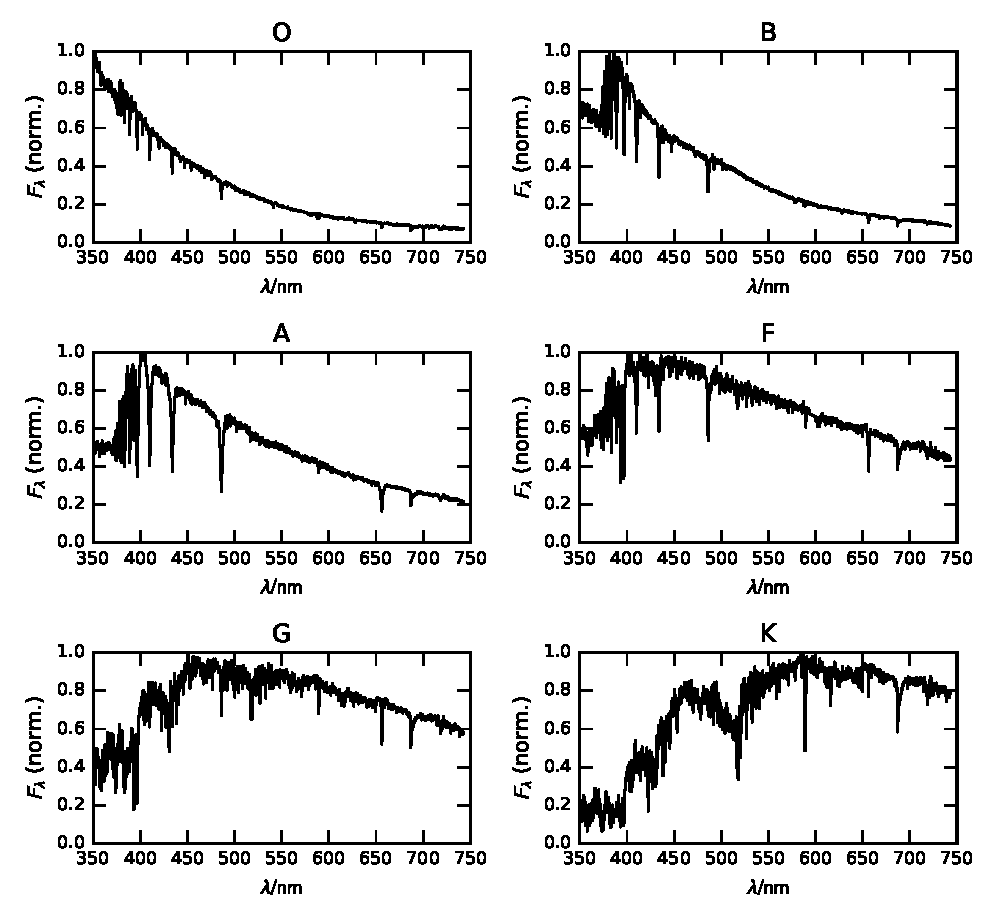
\includegraphics[width=\linewidth]{spectral_types}
\caption[Standard stellar types]{\label{f.spectral-types} Spectra from main-sequence stars of spectral types O--K. Data from \protect\citet{Jacoby1984A-library-of-st}.}
\end{figure}

As we have seen, the temperature of the stellar atmosphere determines which species are present and hence which lines are present. The width of the line conveys information about the pressure at the photosphere. To understand this, we need to digress briefly on the shape of the line.

\begin{sidebar}[The driven damped oscillator]
Let's begin with a simple system: a mass $m$ attached to a spring with force $F = -kx$.

\begin{center}
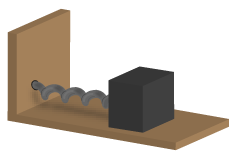
\includegraphics[width=0.5\linewidth]{simple-spring}
\end{center}

\noindent If we put the origin of our coordinate system where the mass is at rest with the spring relaxed, then the equation of motion of the mass is
\begin{equation}\label{e.SHO-basic}
	\DDtt{x} + \frac{k}{m} x = 0.
\end{equation}
You have solved this equation before: the most general solution is
\begin{equation}\label{e.SHO-general-solution}
	x(t) = x_{0}\cos(\wot) + \frac{v_{0}}{\omega_{0}}\sin(\wot)
\end{equation}
with $\omega_{0}^{2} = k/m$ and with $x_{0}$ and $v_{0}$ being the initial position and velocity of the mass. The angular frequency $\omega_{0}$ is related to the period of oscillation $T$ as $\omega_{0} = 2\pi/T$.

\newthought{Now let's push on our mass with an oscillating force, $F\cos(\omega t)$ with $\omega\neq\omega_{0}$.} A real world example would be holding a vibrating tuning fork near another fork tuned to a different frequency.  The equation of motion is now
\begin{equation}\label{e.SHO-driven}
	\DDtt{x} + \omega_{0}^{2}x = \frac{F}{m}\cos(\wt).
\end{equation}
You can verify by substitution that a general solution is
\[
	x(t) = \frac{F/m}{(\omega_{0}^{2}-\omega^{2})}\cos(\wt) + A\cos(\wot)+B\sin(\wot).
\]
Let's start with our harmonic oscillator at rest ($v_{0} = \left.\dif x/\dif t\right|_{t=0} = 0$) and at $\left. x\right|_{t=0} = 0$.  With these conditions, we can determine the constants $A$ and $B$; the solution is
\[
	x(t) = \frac{F/m}{(\omega_{0}^{2}-\omega^{2})}\left[\cos(\wt)-\cos(\wot)\right].
\]
Let's recast this by defining $\Delta = \omega_{0} - \omega$ and $\omega_{m} = (\omega_{0}+\omega)/2$.  Then
\begin{eqnarray*}
  \omega_{0}^{2}-\omega^{2} &=& (\omega_{0}-\omega)(\omega_{0}+\omega) = 2\Delta\omega_{m},\\
  \cos(\wot) &=& \cos\left(\wmt+\Delta t/2\right),\\
  \cos(\wt) &=& \cos\left(\wmt-\Delta t/2\right);
\end{eqnarray*}
using the cosine addition rules and combining terms, we can write the solution as
\begin{equation}\label{e.beats}
	x(t) = \left[\frac{F/m}{\Delta\omega_{m}}\sin(\Delta t/2)\right]\sin(\wmt).
\end{equation}
This illustrates the phenomena of beats: the oscillation consists of a carrier signal at frequency $\omega_{m}$ with the amplitude modulated at the slower frequency $\Delta /2$.  Notice that the amplitude increases as $\Delta \to0$, i.e., $\omega\to\omega_{0}$.

\newthought{Now let's make our model even more realistic by adding some damping.}
We add a frictional force that is proportional to velocity, $F_{\mathrm{friction}} = -m\Gamma \dif x/\dif t$. Our complete equation of motion is then
\begin{equation}
	\DDtt{x} + \Gamma \DDt{x} + \omega_{0}^{2}x = \frac{F}{m}\cos(\omega t).
\end{equation}
The solution to this is straightforward to find, although the algebra is tedious (trust me on this). The general solution for initial conditions $\left.x\right|_{t=0} = x_{0}$ and $\left.\dif x/\dif t\right|_{t=0} = v_{0}$ is
\begin{eqnarray}
\label{e.general-solution-ddo}
\lefteqn{x(t) = \frac{F\womw/m}{\womw^{2}+\gw}\cos(\omega t)} && \\
	&+& \frac{\Gamma\omega F/m}{\womw^{2}+\gw}\sin(\omega t)\nonumber \\
	&+& {\color{red}\left[x_{0}-\frac{F\womw/m}{\womw^{2}+\gw}\right] e^{-\Gamma t/2} \cos(\omega_{\Gamma}t)} \nonumber\\
	&+& {\color{red}\left[\frac{v_{0}}{\omega_{\Gamma}}-\frac{\Gamma\omega F/m}{\womw^{2}+\gw}
	\,\frac{\omega}{\omega_{\Gamma}}\right]e^{-\Gamma t/2} \sin(\omega_{\Gamma}t)}, 
	\nonumber
\end{eqnarray}
with
\[ 
    \omega_{\Gamma} = 
        \omega_{0}\left(1-\frac{\Gamma^{2}}{4\omega_{0}^{2}}\right)^{1/2}.
\]
Let's simplify this a bit.  First, the last two terms decay as $e^{-\Gamma t/2}$: these are transients set by the initial conditions. After a time $t \gg 2/\Gamma$ only the first two terms, which oscillate at the driving frequency $\omega$, will remain. 

We can simplify these first two terms even further: if we write
\[ \cos(\wt) = \frac{e^{i\wt}+e^{-i\wt}}{2},\quad \sin(\wt) 
    = \frac{e^{i\wt}-e^{-i\wt}}{2i}, \]
we can combine them and obtain
\begin{eqnarray}
    x(t) &=& \frac{F}{2m}\left[\frac{1}{\left(\omega_0^2-\omega^2\right) + i\Gamma\omega}\right]e^{i\wt} \nonumber\\
    && + \frac{F}{2m}\left[\frac{1}{\left(\omega_0^2-\omega^2\right) - i\Gamma\omega}\right]e^{-i\wt} \nonumber\\
    &=& \Re\left\{\frac{F}{m}\left[\frac{1}{\left(\omega_0^2-\omega^2\right) + i\Gamma\omega}\right]e^{i\wt}\right\}\label{e.oscillator-expression}
\end{eqnarray}
We use the symbol ``$\Re$'' to denote taking the real part of a complex quantity.
The oscillation can be described as the real part of a complex quantity $Ae^{i\wt}$, with
\[
    A = \frac{F}{m}\left[\frac{1}{\left(\omega_0^2-\omega^2\right) + i\Gamma\omega}\right]
\]
being the (complex) amplitude.
\end{sidebar} 

For $\omega \approx \omega_0$, we write $(\omega_0^2-\omega^2)\approx 2\omega_0(\omega_0-\omega)$ and take the square of the amplitude to find,
\begin{eqnarray}
    \left|A\right|^2 &=& \left(\frac{F}{2m\omega_0}\right)^2
        \frac{1}{(\omega_0-\omega)^2 + (\Gamma/2)^2}\nonumber\\
    &=& \frac{\pi}{2\Gamma}\left(\frac{F}{m\omega_0}\right)^2
        \left\{\frac{1}{\pi}\frac{\Gamma/2}{(\omega_0-\omega)^2 + (\Gamma/2)^2}\right\}
\end{eqnarray}
We rewrote the amplitude in the second line so that the term in $\{\cdot\}$ is normalized. The function
\[
    \mathcal{L}(\omega;\Gamma) = \frac{1}{\pi} 
        \frac{\Gamma/2}{(\omega_0-\omega)^2 + (\Gamma/2)^2}
\]
is known as a Lorentzian.  In contrast to a Gaussian, a Lorentzian is characterized by broad ``wings'' (Fig.~\ref{f.comparison}) as it goes to zero away from the central frequency $\omega_{0}$.
\begin{marginfigure}[-4\baselineskip]
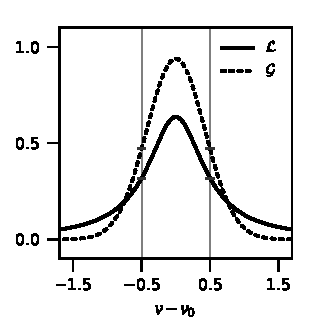
\includegraphics[width=\linewidth]{comparison}
\caption[Comparison of Lorentzian and Gaussian distributions]{\label{f.comparison}
Comparison of a Lorentzian ($\mathcal{L}$, solid line) and a Gaussian ($\mathcal{G}$, dotted line), both with $\mathrm{FWHM}=1$. The area under each curve is unity.}
\end{marginfigure}

\newthought{Consider an electronic transition in an atom between two energy levels, $E_m$ and $E_n$.} The natural frequency of this transition is $\nu_0 = |E_n-E_m|/h$. Light incident on the atom with frequency\sidenote{We are switching from angular frequency $\omega$ to frequency $\nu = \omega/2\pi$.} $\nu\neq\nu_0$ drives the electron at frequency $\nu$. An accelerating electron radiates, which damps the acceleration of the electron.  Classically, the transition in an atom is an electromagnetic oscillator with damping and driving terms, with cross-section\sidenote{For details, see the Box~\ref{b.line-emission}.}
\begin{equation}\label{e.semi-classical}
    \sigma = \left(\frac{\pi e^2}{m_e c}\right)
    \left\{\frac{\Gamma/4\pi}{(\nu_0-\nu)^2 + (\Gamma/4\pi)^2}\right\}.
\end{equation}
The actual value of the cross-section must be calculated using quantum mechanics. The overall shape of the cross-section is still in the form of equation~(\ref{e.semi-classical}) with opacity
\begin{equation}
    \rho\kappa_\nu = n_i \left(\frac{\pi e^2}{m_e c}\right) f_{mn}
        \left\{\frac{\Gamma/4\pi}{(\nu_0-\nu)^2 + (\Gamma/4\pi)^2}\right\}.
\end{equation}
In this equation, $f_{mn}$ is a number, called the \emph{oscillator strength}, that results from the calculation of the transition probability from state $m$ to state $n$, and $n_i$ is the density of atoms in state $m$.  The key point is that $f_{mn}$ depends only on the details of the transition: the energies, spins, and parities of the atomic states.  It does not depend on environmental parameters such as temperature and pressure.  As a result, $f_{mn}$ can be measured or computed once and then tabulated.


\begin{sidebar}[Treating line emission as a driven damped oscillator]
\label{b.line-emission}
NB. In this box, Gaussian CGS units are used for the electromagnetic field. To convert to MKS, make the following substitutions:
\begin{eqnarray*}
e &\to& \frac{1}{\sqrt{4\pi\varepsilon_0}}e\\
\bvec{E} &\to& \sqrt{4\pi\varepsilon_0}\bvec{E}\\
c &\to& (\mu_0\varepsilon_0)^{-1/2}.
\end{eqnarray*}

\newthought{Suppose we have a classical charged harmonic oscillator.}  The instantaneous power emitted by the oscillator is
\begin{equation}\label{e.larmor-power}
	 P(t) = \frac{2}{3}\frac{e^{2}}{c^{3}} |\dot{\vu}|^{2},
\end{equation}
and when averaged over a cycle is
\begin{equation}\label{e.oscillator-power}
	 \left\langle P(t) \right\rangle = \frac{e^{2}}{3c^{3}}x_{0}^{2} \omega^{4},
\end{equation}
since $\dot{\vu} = -\omega^{2}\bvec{x}_{0}\cos \omega t$. Since the oscillator is radiating, it is losing energy and is damped. Let us write the damping as $\bvec{F}_{\mathrm{rad}}\vdot \vu$; to find $\bvec{F}_{\mathrm{rad}}$, we integrate the power loss over a cycle,
\[  -\int_{t_{1}}^{t_{2}}\!\dif t\;\frac{2}{3}\frac{e^{2}}{c^{3}}\dot{\vu}\vdot\dot{\vu} 
	= -\left.\frac{2}{3}\frac{e^{2}}{c^{3}}\dot{\vu}\vdot\vu\right|_{t_{1}}^{t_{2}} 
	+ \frac{2}{3}\frac{e^{2}}{c^{3}} \int_{t_{1}}^{t_{2}}\!\dif t\;\ddot{\vu}\vdot\vu. 
\]
Since the motion is periodic, the first term vanishes and we can therefore identify 
\[ 
	\bvec{F}_{\mathrm{rad}} = \frac{2}{3}\frac{e^{2}}{c^{3}}\ddot{\vu} 
	= -m\left(\frac{2e^{2}\omega^{2}}{3c^{3}m}\right)\vu
\]
as the radiation damping term with the term in parenthesis being the damping constant $\gamma$. 
If there is an driving electric field on our oscillator, then its equation of motion becomes
\begin{equation}\label{e.eq-sho}
	m\ddot{\bvec{x}} = -m\omega_{0}^{2}\bvec{x} + e\bvec{E}e^{i\omega t} - m\gamma \dot{\bvec{x}}.
\end{equation}
Using a trial function $\bvec{x}\propto e^{i\omega t}$ gives
\[
	\bvec{x} = \frac{e}{m}\frac{E e^{i\omega t}}{(\omega_{0}^{2}-\omega^{2}) + i\omega\gamma}.
\]
Taking the second derivative w.r.t.\ time of $\bvec{x}$, substituting into eq.~(\ref{e.larmor-power}), and averaging over a cycle gives the power radiated by the oscillator,
\[
	\left\langle P(t)\right\rangle = \frac{e^{4}\omega^{4} E^{2}}{3 c^{2}m^{2}}
	\frac{1}{(\omega_{0}^{2}-\omega^{2})^{2} + \gamma^{2}\omega^{2}}.
\]
Dividing $\langle P(t)\rangle$ by the incident power per unit area, $cE^{2}/(8\pi)$, gives the cross-section:
\begin{equation}\label{e.classical-oscillator-cross-section}
	\sigma = \frac{8\pi}{3}\frac{e^{4}}{m^{2}c^{3}}
	\frac{\omega^{4}}{(\omega_{0}^{2}-\omega^{2})^{2} + \gamma^{2}\omega^{2}}.
\end{equation}
Now, for $\omega \approx \omega_{0}$, we can expand $(\omega_{0}^{2}-\omega^{2})^{2} \approx 4\omega_{0}^{2}(\omega_{0}-\omega)^{2}$; furthermore, we identify $2e^{2}\omega_{0}^{2}/(3c^{3}m) = \gamma$ and equation~(\ref{e.classical-oscillator-cross-section}) becomes
\begin{equation}\label{e.cross-section-lorentz}
	\sigma = \pi\left(\frac{e^{2}}{mc}\right)\frac{\gamma}{(\omega_{0}-\omega)^{2} + (\gamma/2)^{2}}.
\end{equation}
The line profile is Lorentzian, with a width $\gamma$. In terms of wavelength, the width is
\[ 
	\Delta \lambda = \left|\frac{\dif\lambda}{\dif\omega}\right|\gamma = \frac{2\pi c}{\omega^{2}}\gamma
	= \val{\sci{1.2}{-4}}{\textrm{\AA}}.
\]
This width is independent of the transition frequency (it is just the classical electron radius), and it is very, very small.  In a stellar atmosphere, the width is set by interactions and doppler broadening.

\newthought{To understand how impacts affect the line width}, suppose we model the oscillator as being started and stopped by impacts; in between impacts it just goes as $e^{i\omega_{0}t}$.  To get the spectrum, we take the Fourier transform,
\[
	F(\omega,t) = \int_{0}^{t}\!\dif t'\; \exp[i(\omega_{0}-\omega)t'],
\]
where $t$ is some time between impacts. Now if the impacts are distributed randomly and are uncorrelated, then the distribution of wait times follows a Poisson distribution,
\[ W(t)\,\dif t = e^{-t/\tau}\,\dif t/\tau, \]
where $\tau$ is the average time between collisions.  Using this to compute the energy spectrum, we obtain
\[ E(\omega) = \frac{1}{2\pi\tau}\int_{0}^{\infty}\!\dif t\; F(\omega,t)F^{*}(\omega,t)W(t) = \frac{1}{\pi\tau} 
	\frac{1}{(\omega_{0}-\omega)^{2} + (1/\tau)^{2}};
\]
the line profile is again Lorentzian, with a FWHM $2/\tau$.
\end{sidebar}

\newthought{There is an intrinsic width $\Gamma$ that is set by the finite lifetime of the energy levels;} in practice, however, this is not important.  In a stellar atmosphere, the width $\Gamma$ is set by collisions.  For example, when an electron passes close by our atom, the electric field shifts the energy levels of the atom\sidenote{This is an application of the \emph{Stark} effect that you learn about in quantum mechanics.}.  The greater the collision rate, the larger the width.
If we have two stars of the same photospheric temperature (so that both stars have the same lines), then a way to increase the collision rate is to increase the pressure. Recall, however, that in the stellar atmosphere $P = (g/\kappa)\tau$; as a result, stars with a higher surface gravity will have broader lines. The inset in Figure~\ref{f.compare_grav} illustrates the broadening of the Balmer H$\gamma$ line ($5\to 2$) in the spectrum of a main-sequence A1 star compared with that of a supergiant A1 star.

\begin{figure}[hp]
    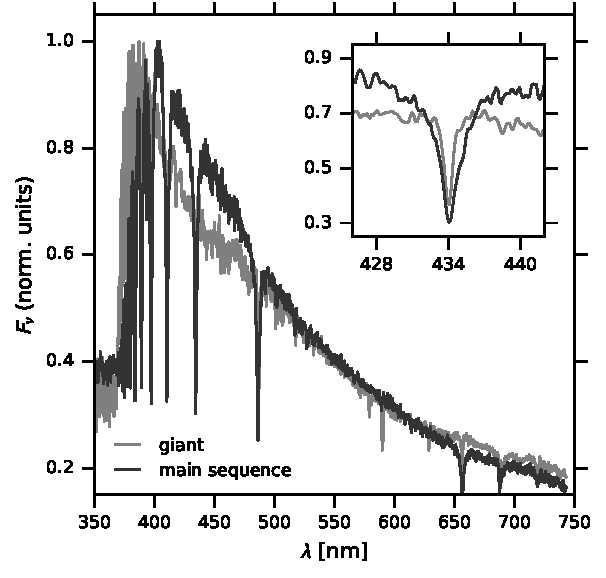
\includegraphics[width=\linewidth]{compare_grav}
    \caption[Spectra of two A1 stars]{\label{f.compare_grav}
    Spectra of two A1 stars, HD 16608 (a main sequence star) and SAO 12149 (a supergiant star).  Spectra are from \citet{Jacoby1984A-library-of-st}.
    }
\end{figure}

In addition to the width set by collisions, the line is also broadened by thermal motion: the atoms are in ceaseless motion; those headed towards us absorb at a blueshifted frequency, while those headed away from us absorb at a redshifted frequency.  Because the atomic velocities follow a Maxwell-Boltzmann distribution, the net effect is to make the core of the line (that is, near the center) assume a Gaussian profile.  Because a Gaussian falls off more quickly than a Lorentzian profile (see Fig.~\ref{f.comparison}), the wings of the line are still determined by the collision rate.

We might be inclined to treat the atoms as hard spheres, but this gives a large $\tau$, or equivalently a narrow line width. We are therefore led to consider longer-range interactions for setting the intrinsic line width. Table~\ref{t.perturbers} lists such interactions. For a given impact parameter, the interaction perturbs the energy levels; by integrating over a distribution of  impact parameters one gets the intrinsic damping. Of course, we should really use a quantum mechanical calculation.  We can scale our cross-section to the classical result (eq.~[\ref{e.cross-section-lorentz}]), however, by writing
\begin{equation}\label{e.cross-section}
	 \sigma_{\nu} = \left(\frac{\pi e^{2}}{m_{e}c}\right) f \phi_{\nu}, 
\end{equation}
where $\phi_{\nu}$ is the line profile (dimension $\sim \Hz^{-1}$) and $f$ is a dimensionless cross-section called the \newterm{oscillator strength}.

\begin{table}[htbp]
\caption{Interactions in stellar atmospheres}\label{t.perturbers}
\begin{tabular}{crcc}
\hline
perturbation & form & source & affects\\
\hline\hline
linear Stark & $C_{2} r^{-2}$ & $e^{-}$, $p$, ions & H (H$\alpha$, H$\beta$, \ldots)\\
quadratic Stark & $C_{4} r^{-4}$ & $e^{-}$ & non-hydrogenic ions\\
van der Waals & $C_{6}r^{-6}$ & atoms, H & most atomic lines, esp.\ in cool stars\\
\hline
\end{tabular}
\end{table}
